\documentclass[a4paper]{article}

%% Language and font encodings
\usepackage[english]{babel}
\usepackage[utf8x]{inputenc}
\usepackage[T1]{fontenc}
\usepackage{mathtools}
\usepackage{graphicx}
\usepackage{subcaption}
\usepackage{float}
\usepackage{a4wide}
\usepackage{amsmath}
\usepackage{rotating}

%% Sets page size and margins
\usepackage[a4paper,top=3cm,bottom=2cm,left=3cm,right=3cm,marginparwidth=1.75cm]{geometry}

\title{DataCom Project}
\author{Alexander Backlund, Sebastian Gustafsson, Siri Göhl, Albin Hjelm}

\begin{document}
\maketitle
\newpage

\section{Project idé}
\subsection{Förslag}
Ett spel där man tävlar 1 mot 1 i reaktionshastighet. Spelarna delar en gemensam
spelplan som när spelet startar är tom. En figur av något slag slumpas fram på
spelplanen och det gäller nu att vara den första som hinner klicka på figuren.
När det är avgjort vem som först klickat på figuren fösvinner den från spelplanen och
dyker upp under den spelares namn som klickade först. Nu är spelplanen återigen tom
och nästa figur slumpas fram och processen återupprepas. Först den till x antal vunna
figurer har vunnit.

\subsection{Delad resurs}
Den delade resursen i spelet är den slumpade figuren som bara en kan få tillgång till
och vi kommer behöva en metod av någon form som kan avgöra vilken spelare som
klickade först. Sedan skriver man till ”permanent storage” med information om
poängställning, vems tur, mm.

\subsection{Uppdatering av globala tillstånd}
Här måste spelplanen och resultaten uppdateras i realtid för båda spelarna.

\subsection{Strategier för eventuella problem}
Vi måste kunna:
\begin{itemize}
\item avgöra vem som klickat först.
\item hantera situationen då två spelare trycker exakt samtidigt.
\item hantera anslutningsproblem.
\item använda lås för att undvika korrumperad data.
\end{itemize}

\subsection{Testning}
Använda oss av minst tre datorer varav två klienter och en host.

\subsection{Designförslag}
\begin{figure}[H]
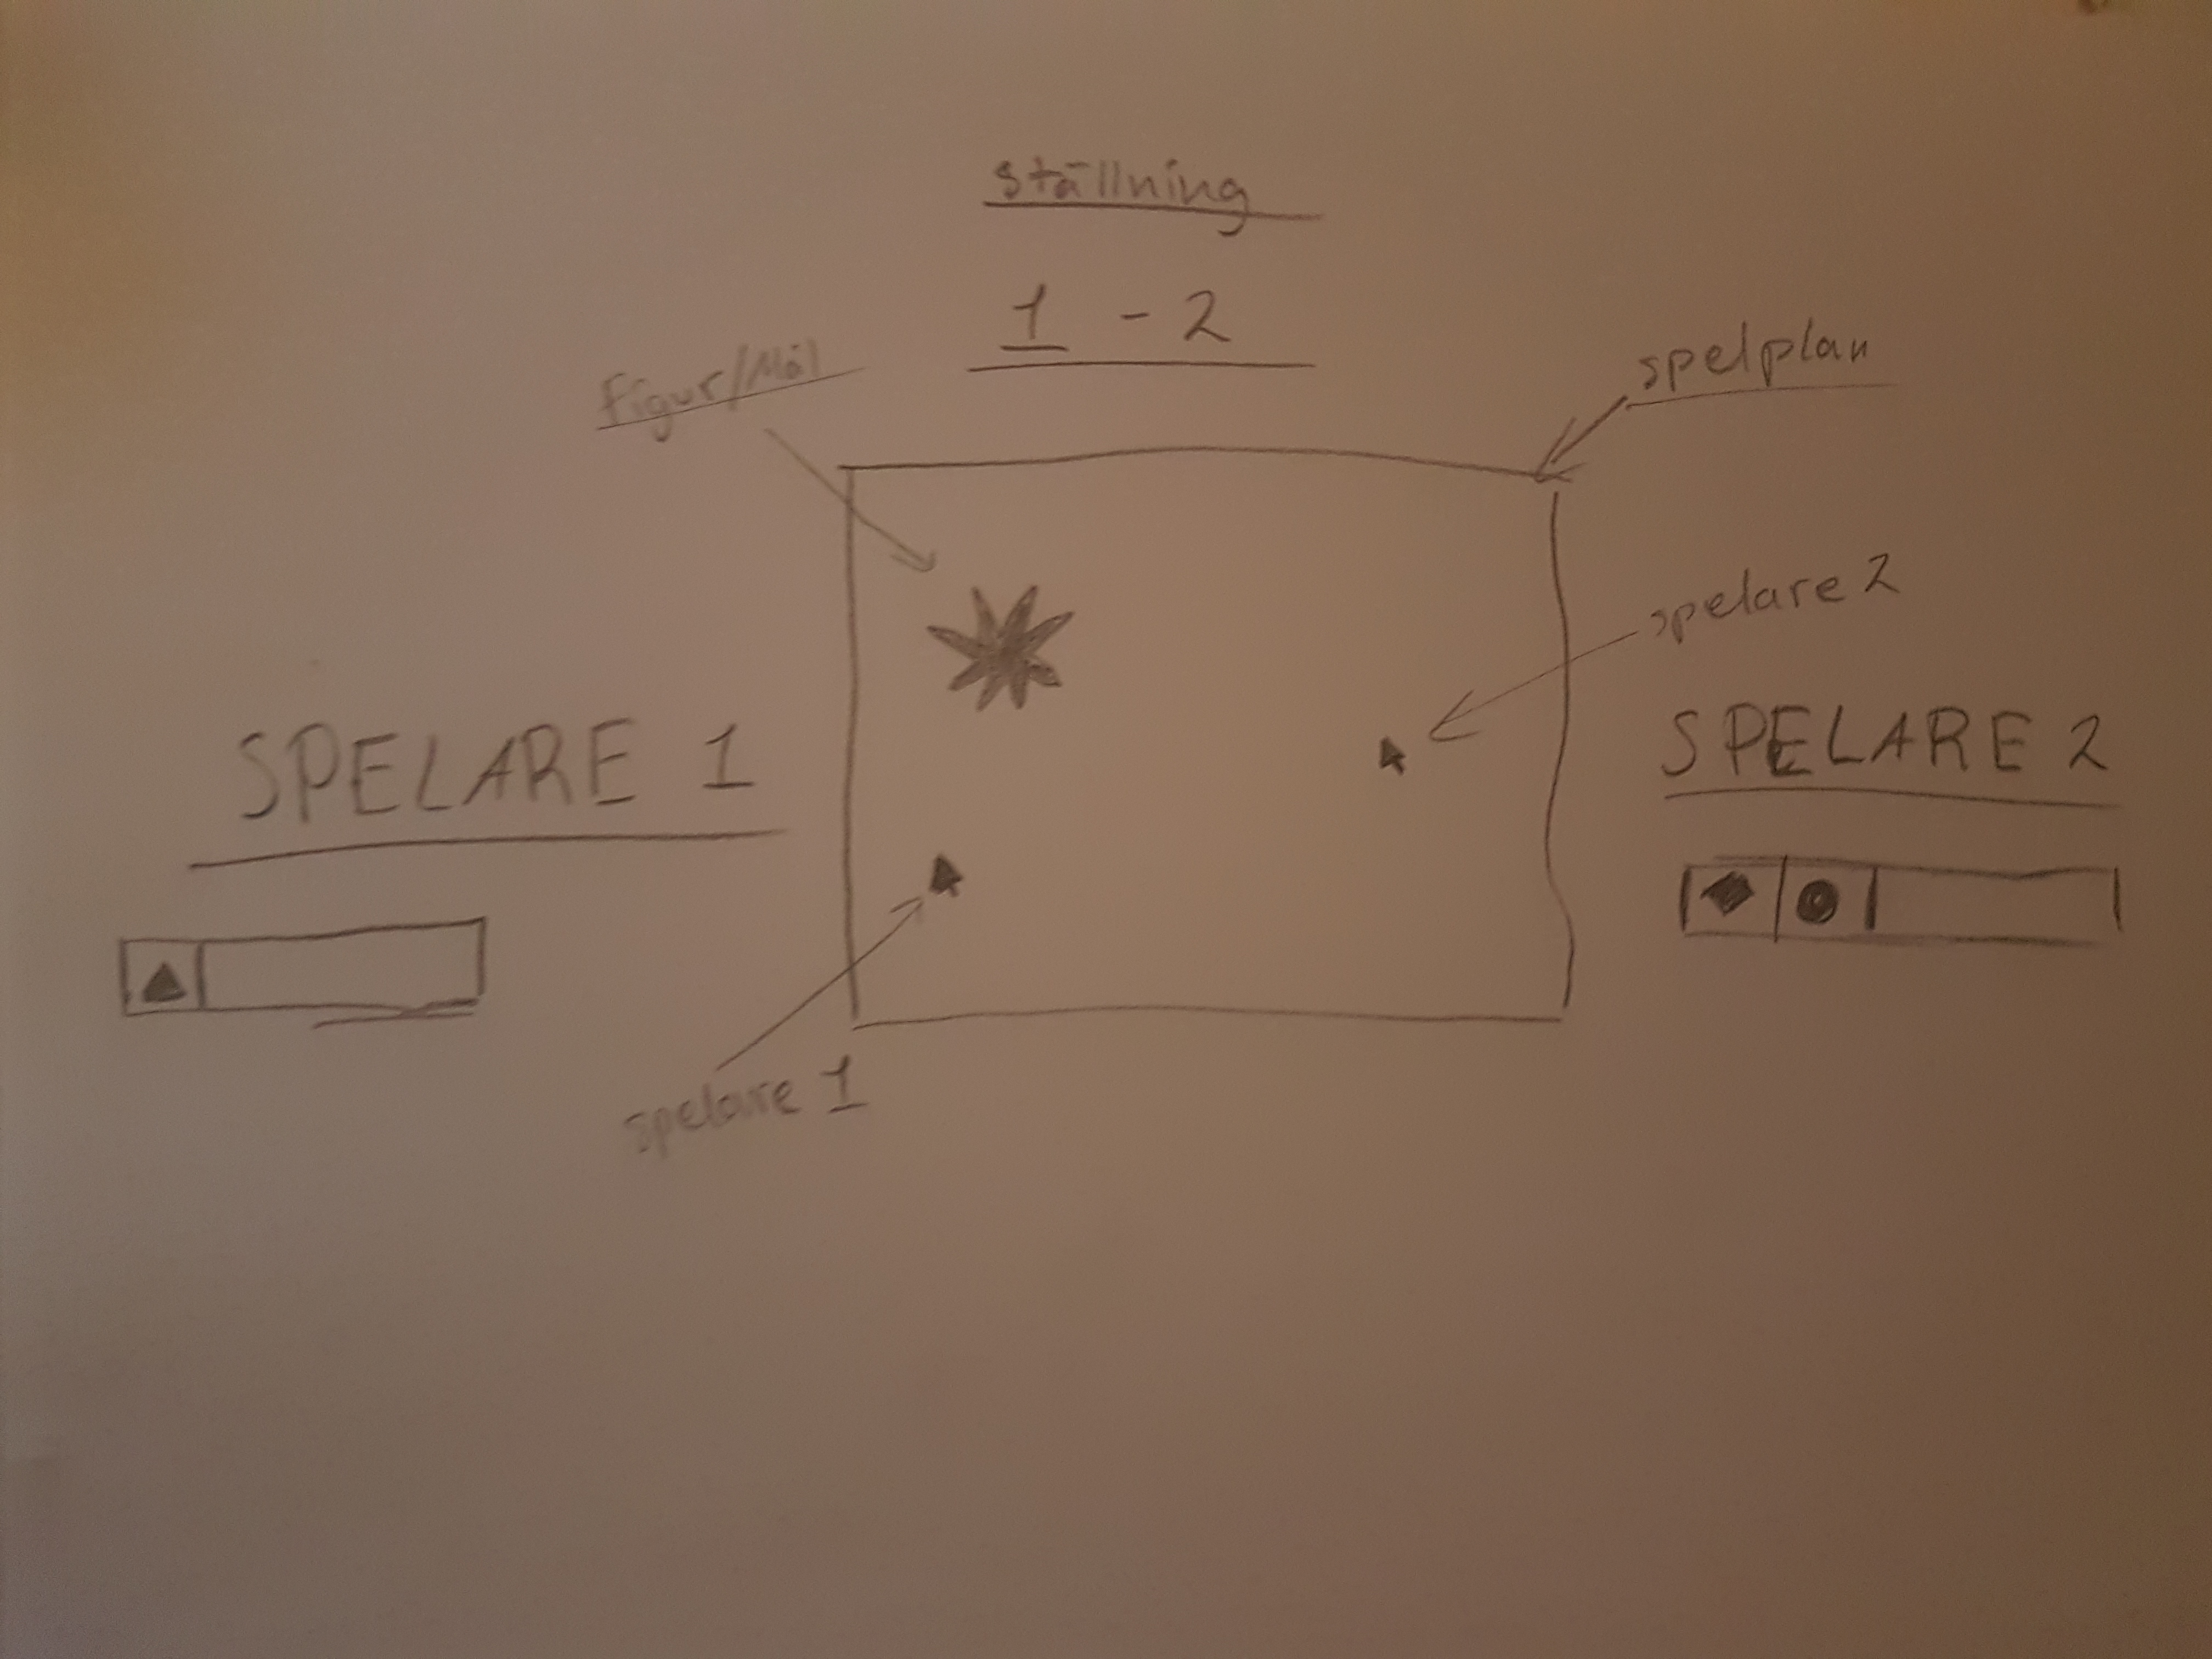
\includegraphics[width=0.8\textwidth]{designf_rslag.jpeg}
\caption{Design förslag}
\end{figure}

Vi kommer implementera systemet i Python, samt använda sockets för kommunikation mellan
systemen.

\subsection{Demonstration av systemet}
Demonstrationen kommer att fokusera på kommunikationen mellan servern och klienten.

\section{System design}
\subsection{Övergripande system design}
\subsubsection{Delar i systemet}
\begin{itemize}
\item klienter
\item Host/server
\item Permanent storage
\end{itemize}

\subsubsection{Hur delarna interagerar med varandra}

\begin{figure}[H]
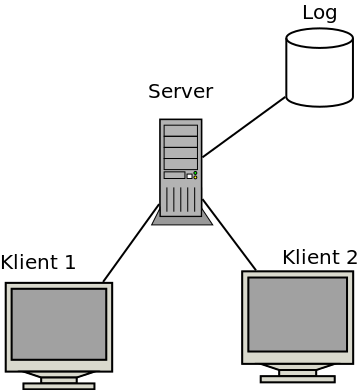
\includegraphics[width=0.8\textwidth]{design.png}
\caption{Hur systemets delar interagerar med varandra}
\end{figure}

\subsubsection{Programmerings miljö}
Vi kommer använda oss av Python och deras socketpaket. Vi använder socketpaketet för att kunna etablera nätverkskanaler mellan servern och klienter. Vi kommer även använda ett grafiskt paket som vi ännu inte har bestämt.
\subsubsection{Problem som kan uppstå}
Vi måste kunna:
\begin{itemize}
\item avgöra vem som klickat först - Tidstämpel hos klienterna.
\item hantera situationen då två spelare trycker exakt samtidigt -  Tidstämpel hos klienterna.
\item hantera om en klients anslutning bryts - Servern hanterar att klienten har förlorat kontakten genom att avsluta spelet och sparar data till permanentat storage.
\item hantera om servern går ner - Servern loggar vinster, förluster. start och avslut av spel. När servern går ner startas servern om och läser av loggen. Om det senaste händelsen inte är avslutat spel då läser servern in ovanstående korrekta händelser.
\item uppnå Kausal ordning - Uppnås genom att använda tidstämplar på kommunikationen från klienterna till servern.
\item kontrollera att tidstämpeln är korrekt -
\end{itemize}


\subsection{Preliminär tidsplan}
\subsubsection{Vad kommer varje medlem göra?}
Vi kommer arbeta i par varav ena paret kommer fokusera på gränssnittet och andra paret kommer att fokusera på server-klient kommunikation. Detta gör vi en vecka åt gången sedan kommer vi rotera i paren. Beroende på tidsåtgång och arbetsbörda får vi efter varje arbetsvecka eventuellt modifiera arbetsuppgifterna för de två grupperna.
\subsubsection{Hur långt kommer vi hinna innan 30:de november?}
Vi försöker sätta upp veckomål, hur lång vi vill ha kommit efter varje vecka. Fram tom. den 30 november vill vi ha et färdigt gränssnitt samt en fungerande klient server kommunikation med de krav tidsstämpling osv. som vi anser viktiga i vår nuvarande bild av systemet. Förhoppningsvis har vi hunnit påbörja integreringen mellan gränssnitt och kommunikationen.

\newpage

\section{Slutgiltiga reflektioner}

\subsection{Vad kunde vi ha gjort bättre?}
Vi skulle kundat ha implementerat stöd för andra språk än engelska, då vi inte hade testat dessa bokstäver i inputen innan redovisningen. Så att programmet inte krashar.\\
\\
Vi borde ha implementerat stöd för om ett packet frösvinner, det skulle kunna varit återsändning alternativt TCP protocol istället för UDP.\\
\\
Vi skulle kunnat implementerat stöd för n-hörningar då vi redan har algoritmen för att bestämma om man klickat i n-hörningen eller inte.

\subsection{Hur har arbetet fortlöpt?}
Arbetet har fungerat bra, vi har arbetat i par, front-end och back-end.
Det har varit bra kommunikation mellan båda paren, om back-end behöver något så fungerade kommunikationen till front-enden väldigt smidigt.

\section{Slutgiltig design}
Ett spel där man tävlar 1 mot N antal spelare i reaktionshastighet. Spelarna delar en gemensam spelplan som när spelet startar är tom. En kvadrat,cirkel eller triangel slumpas fram på spelplanen och det gäller att vara den första som klicka på figuren. Servern skickar vilken tid som figuren ska visas för spelarna, vanligtvis en delay på 3 sek. När en spelare sedan klickar på figuren tar man den aktuella tiden minus den givna tiden då figuren visades. Denna differens skickas sedan till servern som väljer den minsta tiden. Denna spelare får ett poäng.


\end{document}
